\chapter{Практическая часть}
\label{ch:chap2}

\section*{\textbf{Введение}}
На этом занятии отправим в радиоканал мелодию, а потом примем ее и попытаемся воспроизвести.

\section*{\textbf{Конверторы}}

Для отправки мелодии необходимо конвертировать ее из .mp3 в .pcm формат (поток семплов), а потом после принятия конвертировать 
обратно из .pcm в .mp3. Для этого нам понадобятся конверторы. 

\subsection*{\textbf{Из .mp3 в .pcm}}

\begin{lstlisting}
import numpy as np
import librosa
from pydub import AudioSegment

mp3_file = "audio_test.mp3"
pcm_file = "audio_bin.pcm"

# mp3 to pcm
y, sr = librosa.load(mp3_file, sr=44100, mono=True)

pcm_data = (y * 32767).astype(np.int16)

pcm_data.tofile(pcm_file)
\end{lstlisting}

В переменной y хранится массив отсчетов песни, где каждый отсчет принимает значения [-1;1]. sr - частота дискретизации. 
Файл .pcm хранит амплитуды как целые числа от -32768 до 32767, поэтому отмасштабируем значения, домножив их на 32767.

\subsection*{\textbf{Из .pcm в .mp3}}

\begin{lstlisting}
import numpy as np
import librosa
from pydub import AudioSegment

pcm_file = "audio_bin.pcm"
mp3_file = "audio_from_pcm.mp3"

pcm_data = np.fromfile(pcm_file, dtype=np.int16)

audio = AudioSegment(
    data=pcm_data.tobytes(),
    sample_width=2,      # 2 байта = 16 бит
    frame_rate=44100,    # частота дискретизации
    channels=1           # моно
)

audio.export(mp3_file, format="mp3", bitrate="192k")
\end{lstlisting}

Считываем из .pcm файла отсчеты, с помощью функции AudioSegment формируем аудиофайл, а потом сохраняем файл в текущей директории.

\section*{\textbf{Отправка и прием мелодии}}


\subsection*{\textbf{Чтение .pcm файла в C++}}

Чтобы отправить семплы из .pcm файла, нужно для начала считать файл. Для этого напишем функцию

\begin{lstlisting}
int16_t *read_pcm(const char *filename, size_t *sample_count)
{
    FILE *file = fopen(filename, "rb");

    fseek(file, 0, SEEK_END);
    long file_size = ftell(file);
    fseek(file, 0, SEEK_SET);
    printf("file_size = %ld\\n", file_size);
    int16_t *samples = (int16_t *)malloc(file_size);

    *sample_count = file_size / sizeof(int16_t);

    size_t sf = fread(samples, sizeof(int16_t), *sample_count, file);

    if (sf == 0){
        printf("file %s empty!", filename);
    }

    fclose(file);

    return samples;
}
\end{lstlisting}

Передаем в функцию имя .pcm файла и указатель на переменную, в которой потом вернется кол-во считанных семплов. Далее с помощью 
fseek(file, 0, SEEK\_END) перемещаемся в конец файла, а с помощью ftell(file) узнаем текущую позицию в байтах, т.е фактически
узнаем размер файла. Далее выделяем память под массив с семплами, вычисляем кол-во семплов и считываем их из файла.

\subsection*{\textbf{Отправка и прием}}

\begin{lstlisting}
size_t sample_count = 0;
int16_t *samples = read_pcm(PATH_TO_AUDIO, &sample_count);

for (size_t offset = 0; offset < sample_count; offset += 1920 * 2)
{
    if(offset + 1920 * 2 >= sample_count)
        break;

    void *tx_buffs[] = {samples + offset};
    fwrite(samples + offset, 2 * rx_mtu * sizeof(int16_t), 1, tx_data);
    printf("offset: %d", offset);
    flags = SOAPY_SDR_HAS_TIME;
    int st = SoapySDRDevice_writeStream(sdr, txStream, (const void * const*)tx_buffs, tx_mtu, &flags, tx_time, timeoutUs);
    if ((size_t)st != tx_mtu)
    {
        printf("TX Failed: %in", st);
    }        
} 
\end{lstlisting}

Переменная samples содержит семплы, считанные из .pcm файла. Далее запускаем цикл, где будем итерироваться по сдвигам от 0 до 
sample\_count с шагом 1920 * 2 (потому I и Q занимают 2 байта). Сдвиг нужен потому, что за раз отправить мелодию мы не можем,
поскольку размер отправляемого буфера должен составлять 1920 семплов. Далее сделаем проверку на выход за границы массива, чтобы не возникало
ошибок (часть семплов срежется, но на качество это не влияет). Далее формируем tx\_buffs как samples + offset, т.е каждый раз
будем перемещаться по массиву и отправлять следующий блок данных. Прием данных остался неизменным. После выполнения программы
получим семплы мелодии, принятой из радиоканала. Далее конвертируем .pcm файл в .mp3 и наслаждаемся мелодией.

\section*{\textbf{Эксперимент}}

SDR всех студентов работают на одной частоте, соотвественно они создают помехи друг для друга. Возьмем разные мелодии, поставим
SDR рядом и запустим отправку. 

\begin{figure}[H]
    \centering
    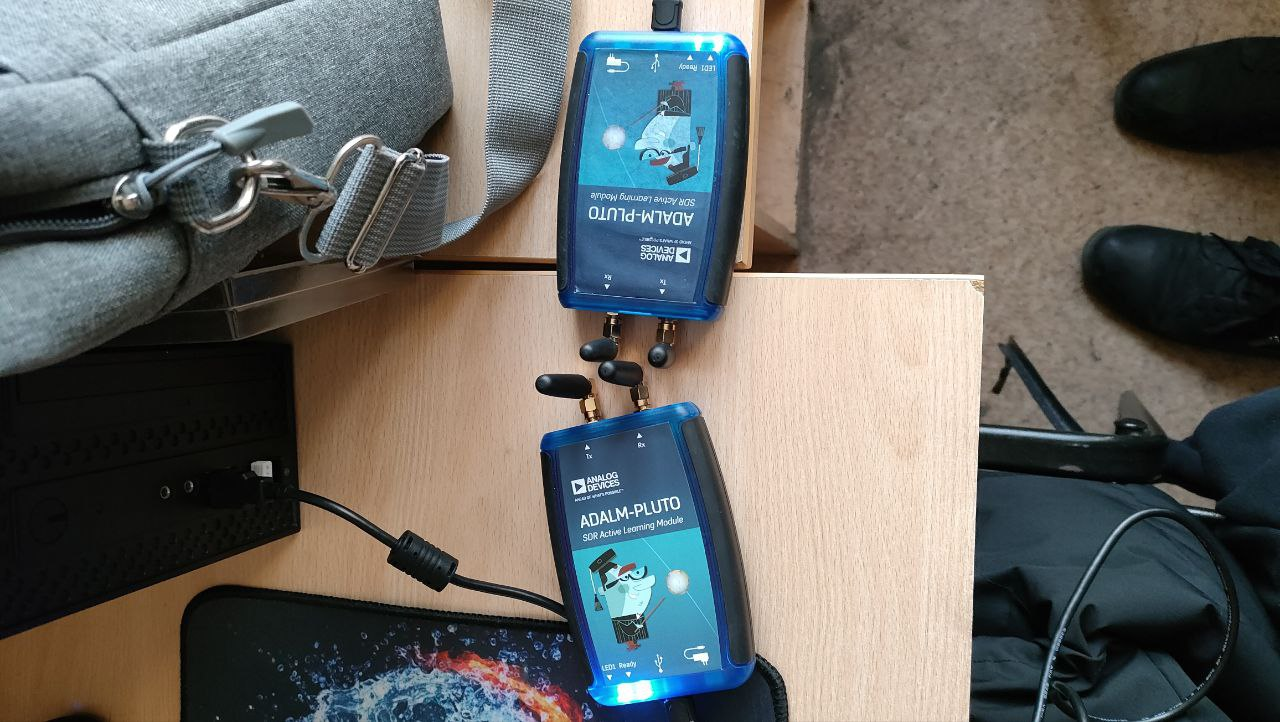
\includegraphics[width=1.0\textwidth]{exp.png}
    \caption{Эксперимент}
\end{figure}

Итоговая мелодия одновременно похожа на две мелодии с некоторыми помехами. Этот пример иллюстриурет недостаток систем
аналоговой связи - она подвержена интерференции от других сигналов.

\section*{\textbf{Реализация логики формирующего фильтра}}

В теории был указан корректный метод для формирования длящихся символов I(t) и Q(t) из символов I и Q. Реализуем эту логику на
Python:

\begin{lstlisting}
    # samples on symbol
    L = 1000

    # samples
    I_upsampling = []
    Q_upsampling = []

    # upsampling for In-phase component
    for x in I_symbols:
        I_upsampling.append(x)
        I_upsampling.extend([0] * (L-1))

    # upsampling for Quadrature component
    for x in Q_symbols:
        Q_upsampling.append(x)
        Q_upsampling.extend([0] * (L-1))
    
    # set impulse response (rect)
    g = [1] * L

    s_I = []
    s_Q = []

    # compute convolution
    for n in range(len(I_upsampling)):
        tmp_I = 0
        tmp_Q = 0
        for m in range(L):
            if n - m >= 0:
                tmp_I += I_upsampling[n-m]*g[m]
                tmp_Q+= Q_upsampling[n-m]*g[m]
        s_I.append(tmp_I)
        s_Q.append(tmp_Q)

\end{lstlisting}

Считывем и парсим из файла символы I и Q. После этого повышаем их частоу дискретизации путем формирования нового списка символов
с добавлением L-1 нулей после каждого. Далее устанавливаем импульсную характеристику сигнала g. Далее вычисляем свертку. В переменных
s\_I и s\_Q находятся символы I(t) и Q(t), растянутые во времени. \\

Для проверки корректности работы визуализируем полученные результаты. Если всё верно, то графики должны быть идентичны графикам
из предыдущего занятия.

\begin{figure}[H]
    \centering
    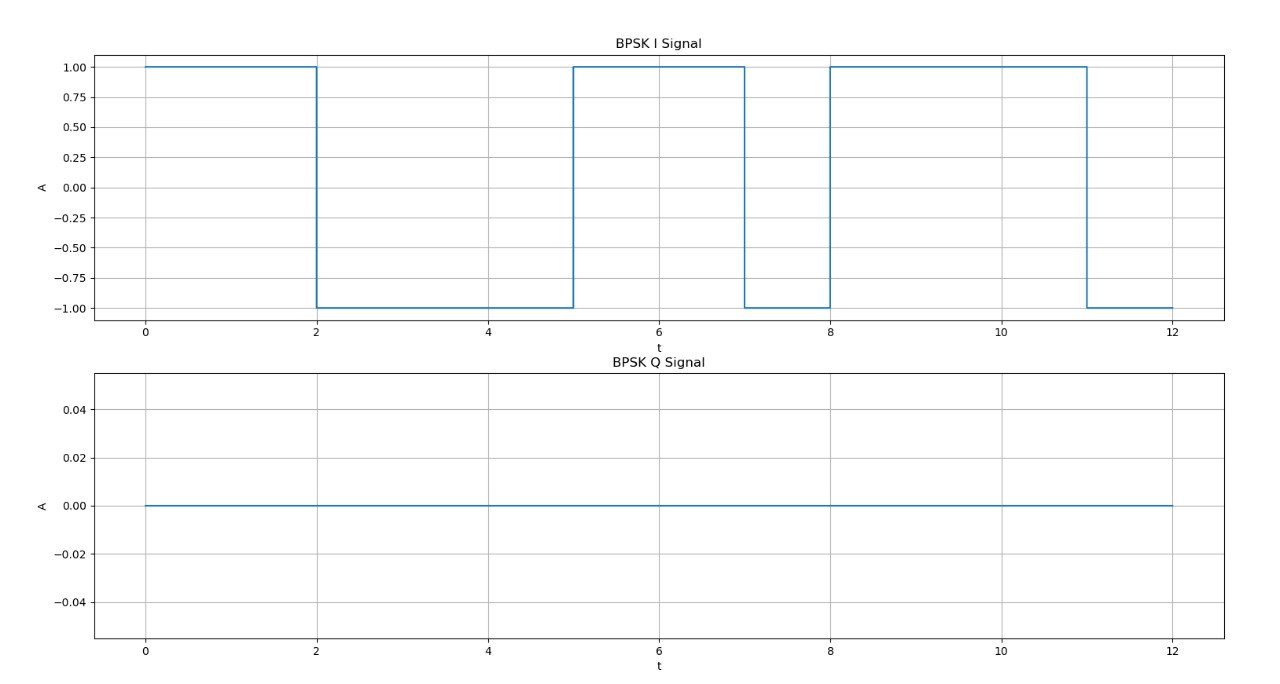
\includegraphics[width=1.0\textwidth]{bpsk_rect.png}
    \caption{Символы во времени (BPSK)}
\end{figure}

\begin{figure}[H]
    \centering
    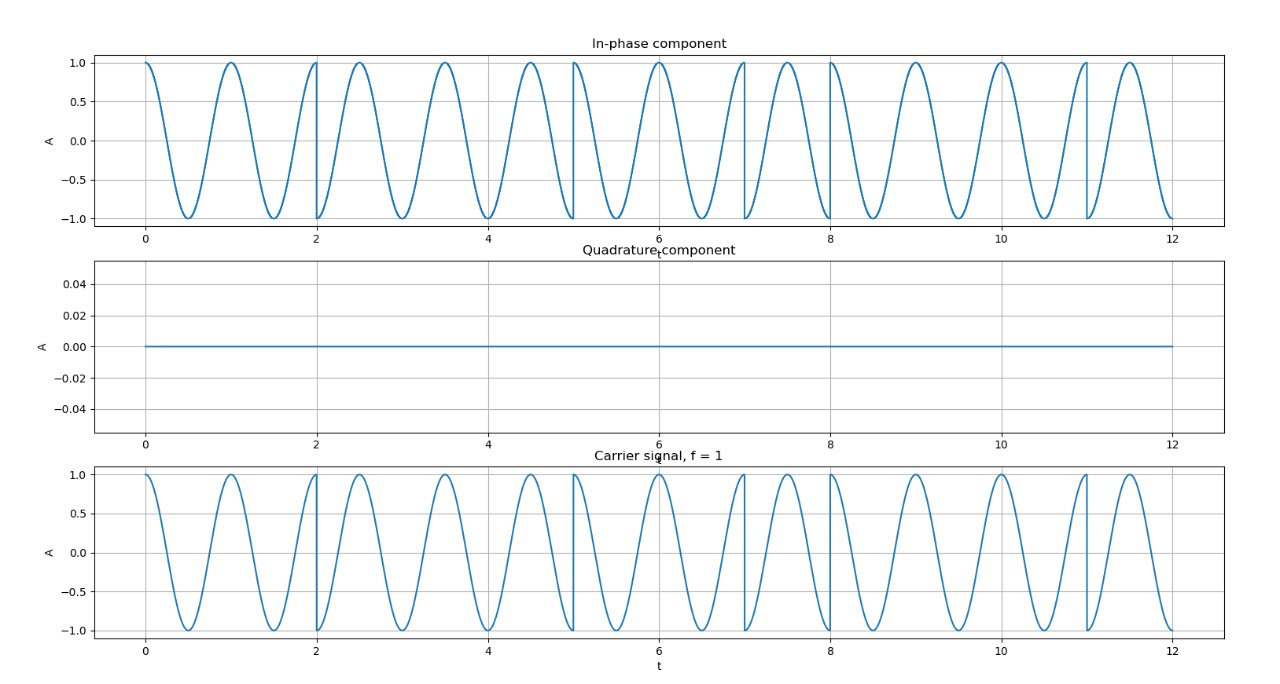
\includegraphics[width=1.0\textwidth]{bpsk_signal.png}
    \caption{Несущее колебание, перемноженное на символы (BPSK)}
\end{figure}


\begin{figure}[H]
    \centering
    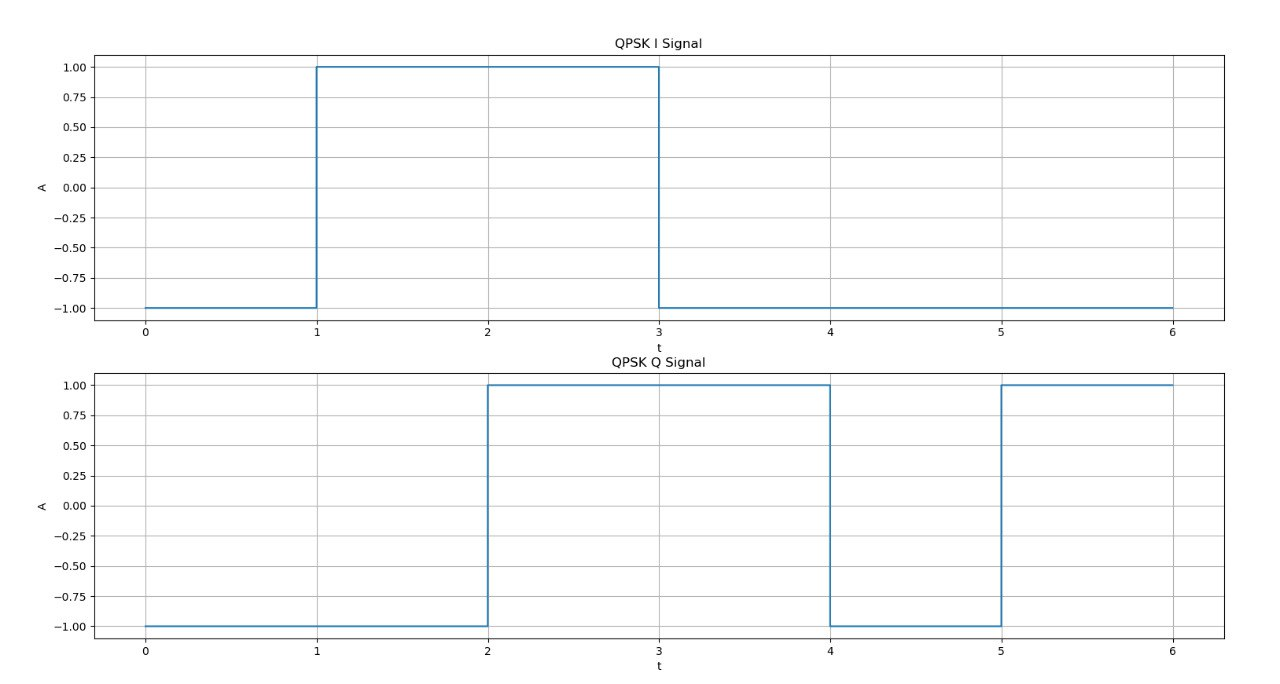
\includegraphics[width=1.0\textwidth]{qpsk_rect.png}
    \caption{Символы во времени (QPSK)}
\end{figure}

\begin{figure}[H]
    \centering
    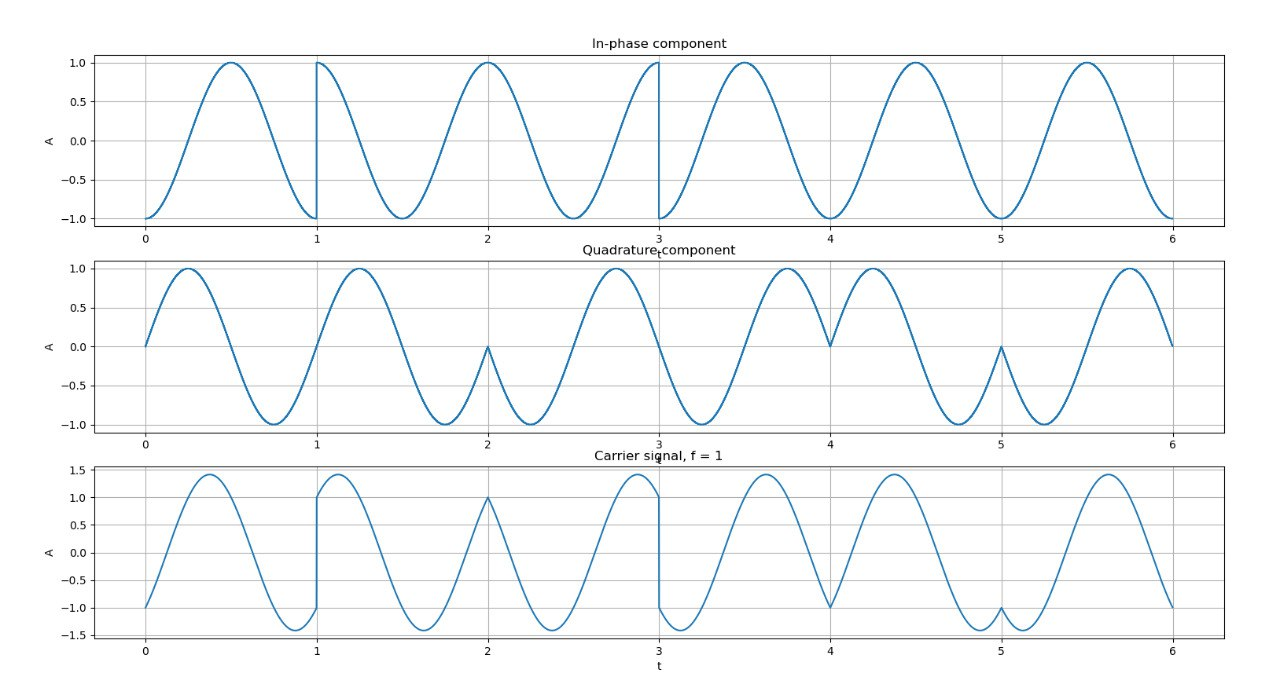
\includegraphics[width=1.0\textwidth]{qpsk_signal.png}
    \caption{Несущее колебание, перемноженное на символы (QPSK)}
\end{figure}

Графики идентичны графикам из прошлого занятия, значит, все работает верно. Таким образом теперь мы можем задать сигналу
любую форму, изменяя импульсную характеристику g. 


\endinput
